Como es parte de la Estadistica descriptiva, tiene como objetivo obtener informacion desde una muestra,
que permita entender o forumular hipotesis acerca del fenomeno que se estudia.

\subsection{Analisis Estratificado}
	El análisis estratificado pretende mostrar cómo cambia una variable (Y) cuando cambia otra (X)
	\begin{itemize}
		\item Se divide una muestra de acuerdo al valor de una variable que llamaremos variable estratificadora X
		\item Se estudia el comportamiento de otra variable  de interés Y (dependiente) en cada subgrupo o estrato
		\item Se da cuenta de cómo cambia el comportamiento de Y al cambiar de estrato X
		\item si la variable explicativa (X) es continua, definir categorías de valores posibles y separar la muestra de acuerdo a ellas
		\item Habiendo estratificado con algún criterio, medimos $\rightarrow$ frecuencias,tendencias(media, mediana,etc),dispersion(IQR)
		\item Habiendo estratificado y analizado el comportamiento de la variables por estrato$\rightarrow$ graficos, box-plots(por cada estrato)
		\item Una forma de medir el efecto de la variable presuntamente explicativa (X) sobre la explicada (Y) es el \emph{An\'alisis de Varianza}.
		\item \textbf{Idea:} si la variable estratificadora X explica bien la otra variable Y, Y no debiera variar mucho con un X constante.
	\end{itemize}
\subsubsection{Analisis de Varianza}
	\begin{itemize}
		\item Varianza Intra-Estratos(dentro de los grupos)$\ =\ \sum_{h=1}^{m}p_{h}\cdot V_{h}$, (frecuencia por varianza)
		\begin{itemize}
			\item ponderamos por el peso del estrato!!!
			\item Varianza no explicada por la variable estratificadora
		\end{itemize}
		\item Varianza Inter-Estratos(dentro de los grupos)$\ =\ \sum_{h=1}^{m}p_{h}\cdot(\bar{Y}_{h}-\bar{\bar{Y}})^{2}$
		\begin{itemize}
			\item media de cada grupo inducido por la variable explicativa X, $\bar{\bar{Y}}\ =\ \sum_{h=1}^{m}p_{h}\cdot\bar{Y}_{n}$
			\item media total o promedio ponderado de las medias por grupo.
		\end{itemize}
		\item Varianza Muestral Total:
		\begin{itemize}
			\item $V_{T}\ =\ \frac{1}{n}\sum_{i}(Y_{i}-\bar{Y})^2$ (Varianza Muestral Sin Estratificar)
			\item $V_{T}\ =\ \sum_{h=1}^{m}p_{h}\cdot V_{h}\ +\ \sum_{h=1}^{m}p_h(\bar{Y}_{h}-\bar{\bar{Y}})^{2}$
			\item $V_{T}\ =\ V_{intra}\ +\ V_{inter}$
		\end{itemize}
		\item Cuociente de Varianza Explicada:
		\begin{itemize}
			\item $\frac{V_{T}}{V_{inter}}$
			\item Medida de la calidad de la variable estratificadora X como variable explicativa para Y\\
			\item Para todo lo anterior necesitamos que Y sea continua, pero X puede ser continua o discreta, numérica o cualitativa.\\\\
		\end{itemize}
	\end{itemize}
	\textbf{Ejemplo:}
	Consideremos la siguiente hip\'otesis de estudio: Caminar ayuda a mantener un \'indice de grasa corporal adecuado.\\
	Para validar la hip\'otesis se tom\'o una muestra de 16 hombres, encuest\'andolos acerca del n\'umero de horas caminadas
	a la semana y midiendo su \% de grasa corporal. La muestra es la siguiente:\\
	\begin{center}
		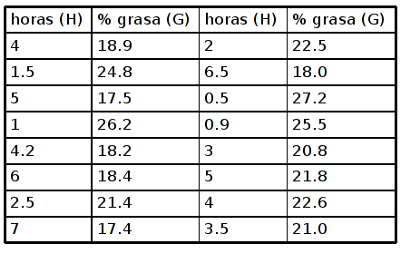
\includegraphics[height=4.5cm]{images/cap3_ej1_1}
	\end{center}
	$$\bar{G}\ =\ 21.3875$$
	$$V_{T}\ =\ 9.7898,\ Calculado\ mas\ adelante$$
	Decidimos estratificar la muestra de acuerdo al número de horas caminadas, considerando 3 clases para el conjunto de valores de esta variable:\\
	$$R\ =\ (7-0.5)\ =\ 6.5$$
	$$A\ =\ (R + 1)/3\ =\ 2.5$$
	\begin{center}
       		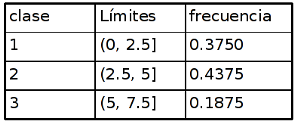
\includegraphics[height=3cm]{images/cap3_ej1_2}
       	\end{center}
	Estratificamos por cada clase de valores para la variable “horas caminadas” generandose 3 submuestras\\
	\begin{center}                                           	
       		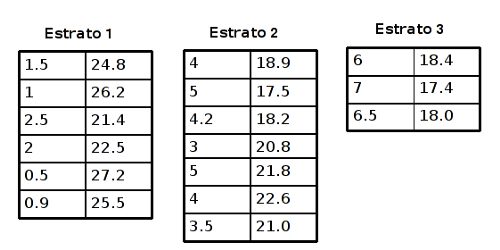
\includegraphics[height=4.5cm]{images/cap3_ej1_3}
        \end{center}
	Medimos las medias y las varianzas por estrato:\\
	\begin{center}                                           	
        	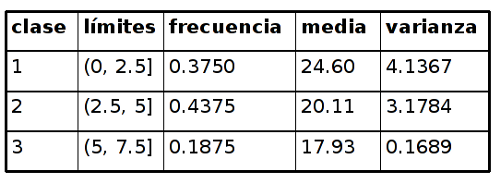
\includegraphics[height=3cm]{images/cap3_ej1_4}
        \end{center}
	Calculamos la varianza intra:
	$$V_{intra}\ =\ 0.375\cdot 4.1367\ +\ 0.4375\cdot 3.1784\ +\ 0.1875\cdot 0.1689$$
	$$V_{intra}\ =\ 2.9735$$
	Calculamos la varianza inter:
       	$$V_{inter}\ =\ 0.375\cdot (24.60\ -\ \bar{G})^2\ +\ 0.4375\cdot (20.11\ -\ \bar{G})^2\ +\ 0.1875\cdot (17.93\ -\ \bar{G})^2$$
       	$$V_{inter}\ =\ 6.8255$$
	Corroboramos la decomposicion propuesta:
	$$V_{T}\ =\ V_{intra}\ +\ V_{inter}\ =\ 2.9735\ +\ 6.8255\ =\ 9.7898$$
	$$\frac{V_{inter}}{V_{T}}\ =\ 0.6966\ \approx 70\%$$
	$$\therefore \ Hay\ una\ relacion\ bien\ significativa$$


	\emph{?`Es valida la relaci\'on entre las varianzas cuando estas se calculan normalizando la suma de cuadrados por n-1 en vez de n?}
	\begin{itemize}
		\item Cuando entremos en Estad\'istica Inferencial justificaremos porqu\'e es m\'as \'uil y correcto comparar las sumas de cuadrados
		\item $S_{T}\ =\ \sum_{I}(Y_{i}-\bar{Y})^{2}$
		\item $S_{intra}\ =\ \sum_{k=1}^{m}\sum_{i\epsilon E_{k}}(Y_{i}-\bar{Y}_{k})^2$, Suma sobre las observaciones del estraro K
		\item $S_{inter}\ =\ \sum_{k=1}^{m}(\bar{Y}_{k}-\bar{Y})^{2}$, suma sobre los estratos
	\end{itemize}
\subsubsection{Analisis de Varianza (ANOVA)}
	Comparamos la variabilidad intra versus la inter.
	\begin{itemize}
		\item $F\ =\ \frac{\frac{S_{inter}}{m-1}}{\frac{S_{intra}}{n-m}}$
		\item \emph{Estad\'istico F de Fisher (m: n\'umero de clases)}
		\item De acuerdo al valor de F podemos aseverar que la variable estratificadora induce cambios en la otra variable con una significancia estadística $\alpha$
	\end{itemize}
\subsection{An\'alisis de Contingencia o Correspondencia}
	\begin{itemize}
		\item  Dadas dos variables X, Y dividir los posibles valores de X en k grupos y los posibles valores de Y en s grupos.
		\item  Determinar luego las frecuencias conjuntas de cada par formado por uno de los grupos de X y uno de los grupos
		 para Y: con qué frecuencia las observaciones caen en un grupo X y un grupo Y simultáneamente.
		\item consta de una tabla que se realiza con las frecuencia con que en la muestra aparecen observaciones que caen en le categoria
		i de acuerdo al valor X y en la categoria j de acuerdo al valor Y
		\item \emph{Frecuencias Marginales:} (sumar todas las frecuencias y ponerlas al final de cada fila y columna)Cuando interesa la frecuencia de una de
		 las variables independiente de lo que pase con la otra  hablamos de Frecuencia Marginal de la variable X \'o Y
		\begin{itemize}
			\item $n_{i\cdot}\ =\ \sum_{j=1}^{s}n_{ij}$ Frecuencia Absoluta de la clase $A_{i}$, Frecuencias Independientes de las clases $B_{j}$
			 a la que estén asociadas: suma de los valores de la fila i-\'esima 
			\item  $n_{\cdot j}\ =\ \sum_{i=1}^{r}n_{ij}$ Frecuencia Absoluta de la clase $B_{j}$, Frecuencias Independientes de las clases $A_{i}$
			 a la que estén asociadas: suma de los valores de la columna j-\'esima 
		\end{itemize}
		\item \emph{Frecuencias Relativas Marginal:} lo mismo que la Marginal solo que cada valor se divide por el total de las muestras.
		\item \emph{Frecuencias Condicionales:} Las frecuencias condicionales de una clase $A_i$ (asociada a X) dado un grupo $B_j$
		 (asociado a Y) corresponden a la proporci\'on de casos de $B_j$ en que se observa $A_i$ y viceversa.
		\begin{itemize}
			\item $f_{i/j}\ =\ \frac{n_{ij}}{n_{\cdot j}}\ =\ \frac{f_{ij}}{f_{\cdot j}}$
			\item $f_{j/i}\ =\ \frac{n_{ij}}{n_{i\cdot}}\ =\ \frac{f_{ij}}{f_{i\cdot}}$
			\item Si se quiere condicionar a X o Y, lo que se tiene que hacer es dividir cada valor de la tabla, por la frecuencia
			 marginal de su columna(Y) o fila(X)
			\item Proporcionan una forma de medir la influencia de la variable X sobre la variable Y (o viceversa)
			\item Notar que las frecuencias se normalizan por un n\'umero m\'as reducido de casos, que corresponden a los 
			casos en que se observa el condicionante. 
		\end{itemize}
		\item \emph{Independencia}
			\begin{itemize}
				\item Diremos que X es independiente de Y si las frecuencias condicionales de X a las diferentes clases de Y son
				 todas iguales; es decir, no dependen de la clase condicionante:(y viceversa)
				$$f_{i/1}\ =\ f_{i/2}\ =\ \ldots\ =\ f_{i/s}\ \forall i$$
				$$f_{j/1}\ =\ f_{j/2}\ =\ \ldots\ =\ f_{j/r}\ \forall j$$
				\item Observaciones:
				\begin{itemize}
					\item Si X es independiente de Y: $f_{i/j}\ =\ f_{i\cdot}\ ,\forall i,j$
					\item Si Y es independiente de X: $f_{j/i}\ =\ f_{\cdot j}\ ,\forall i,j$
					\item Si X es independiente de Y: $f_{ij}\ =\ f_{i\cdot}\ \cdot\ f_{\cdot j}$
					 $$Dem:\ f_{i/j}\ =\ \frac{n_{ij}}{n_{\cdot j}}\ =\ \frac{f_{ij}}{f_{\cdot j}}\ \rightarrow f_{ij}\ =\ 
					f_{i/j}\cdot f_{\cdot j}\ =\ f_{i\cdot}\cdot f_{\cdot j},\ \forall i,j$$
					\item Si X es independiente de Y entonces Y es independiente de X: 
					$$f_{j/i}\ =\ \frac{f_{ij}}{f_{i\cdot}}\ =\ \frac{f_{ij}}{\frac{f_{ij}}{f_{\cdot j}}}$$
				\end{itemize}
				\item \emph{Informaci\'on Mutua:} 
				\begin{itemize}
					\item Si aceptamos la tabla de contingencia como una distribuci\'on aproximada podemos
					 computar la información mutua de X e Y.
					\item  Si X es independiente de Y, I=0 y  Si X = Y, I es equivalente a la entropía de X
					\item $I(x,y)\ =\ \sum_{i,j}f_{ij}\log\left(\frac{f_{ij}}{f_{i\cdot}\cdot f_{\cdot j}}\right)$
				\end{itemize}
			\end{itemize}
	\end{itemize}
